\documentclass[12pt,a4paper]{report}
\usepackage[utf8]{inputenc}
\usepackage[spanish]{babel}
\usepackage{amsmath}
\usepackage{amsfonts}
\usepackage{amssymb}
\usepackage{makeidx}
\usepackage{graphicx}
\usepackage[hidelinks]{hyperref}
\usepackage[left=2cm,right=2cm,top=2cm,bottom=2cm]{geometry}



\begin{document}

\author{Cesar Omar Alvarado Contreras\\
Marco Manzo Torrez\\
Eduardo Robles Vazquez\\
Victor Gabriel Tapia Casillas\\
Fonseca Camaarena Jonathan}

\title{\begin{center}

\includegraphics[scale=1.5]{Escudo.png} 
\end{center}Instalación de ROS}

\date{
Universidad Politécnica de la Zona Metropolitana de Guadalajara\\
Profesor: Carlos Enrique Morán Garabito\\
19 de septiembre del 2019}

\maketitle
\tableofcontents
\section{Introducción}
ROS, es un conjunto de bibliotecas de software y herramientas que ayudan a crear aplicaciones roboticas. Desde controladores hasta algoritmos del estado del arte y con potentes herramientas de desarrollo, ROS tiene lo que necesitas para tu próximo proyecto de robótica. 

\noindent Entre sus fortalezas está que es usado en investigación, productos comerciales, educación y como centro de entretenimiento, tanto en el sector academico y el sector privado.

\noindent En este apartado, aprenderemos a realizar la instalación de ROS en el sistema operativo ubuntu, descargaremos las bibliotecas necesarias para el funcionamiento y creación de campo de trabajo en nuestra computadora.
\section{preparación para instalación}
Primeramente como parte de la instalación, tenemos que configurar nuestro dispositivo para aceptar el software y todos los paquetes de ros.

\begin{figure}[h]
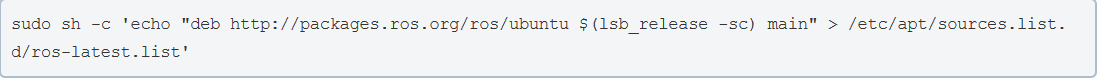
\includegraphics[scale=.8]{link1.png}
\end{figure}

preparamos las llaves de nuestro sistema Ubuntu, como segunda parte del proceso

\begin{figure}[h]
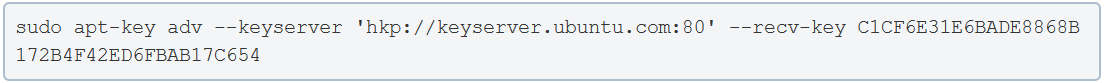
\includegraphics[scale=.8]{link11.png}
\end{figure}

\section{instalación}
procedemos a la instalación de ros, como primer paso nos aseguramos de que nuestro sistema Ubuntu se encuentra actualizado, para ello lanzamos el siguiente código.
\begin{figure}[h]
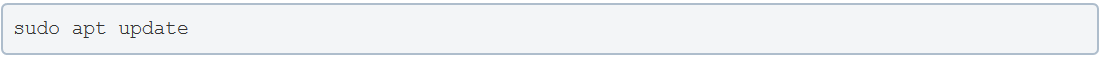
\includegraphics[scale=.8]{link20.png}
\end{figure}
Hay muchas herramientas diferentes en ROS. Se proporciona la configuración básica para que pueda comenzar. 
A continuación tenemos los elementos seleccionados y configuraciones recomendadas
Instalación completa en el escritorio: (recomendado) : ROS, rqt , rviz , bibliotecas genéricas de robots, simuladores 2D / 3D y percepción 2D / 3D\\

\begin{center}
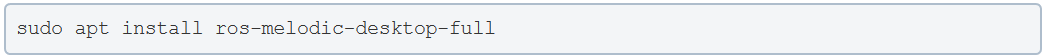
\includegraphics[scale=.8]{link13.png}
\end{center}

Para encontrar paquetes disponibles después de realizar la instalación, usamos el siguiente código:

\begin{center}
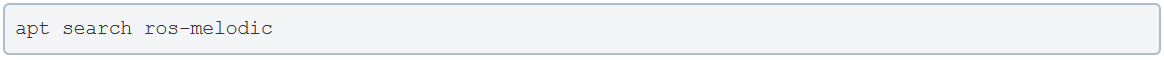
\includegraphics[scale=.8]{link15.png}
\end{center}
como siguiente paso instalamos rosdep para encontrar fácilmente las dependencias y componentes de ros.

\begin{center}
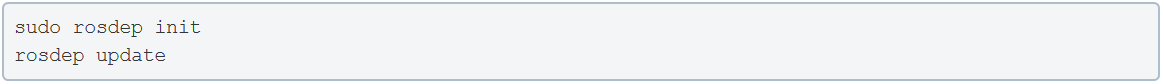
\includegraphics[scale=.8]{link16.png}
\end{center}

\section{declaración de entorno de trabajo}
Declaramos el archivo setup.bash
Si se tienen varias versiones de ros, se creará un conflicto con el archivo setup.bash, por lo que solo se recomienda una versión y una configuración del archivo setup.bash
después de esto, ya tenemos listo nuestro ambiente de trabajo. la instalación ha finalizado y solo falta realizar la comprobación de la correcta instalación.

\begin{figure}[h]
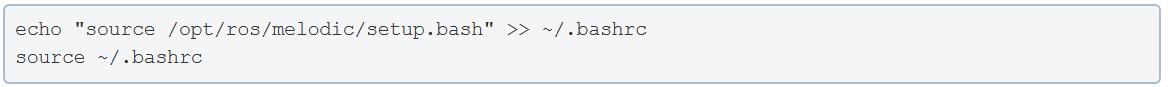
\includegraphics[scale=.8]{link17.png}
\end{figure}

\section{Comprobación de instalación}
lanzamos el complemento roscore para verificar que la instalación se realizó con exito, nos aparecerá de la siguiente manera (si no se tuvo ningún error).

\begin{center}
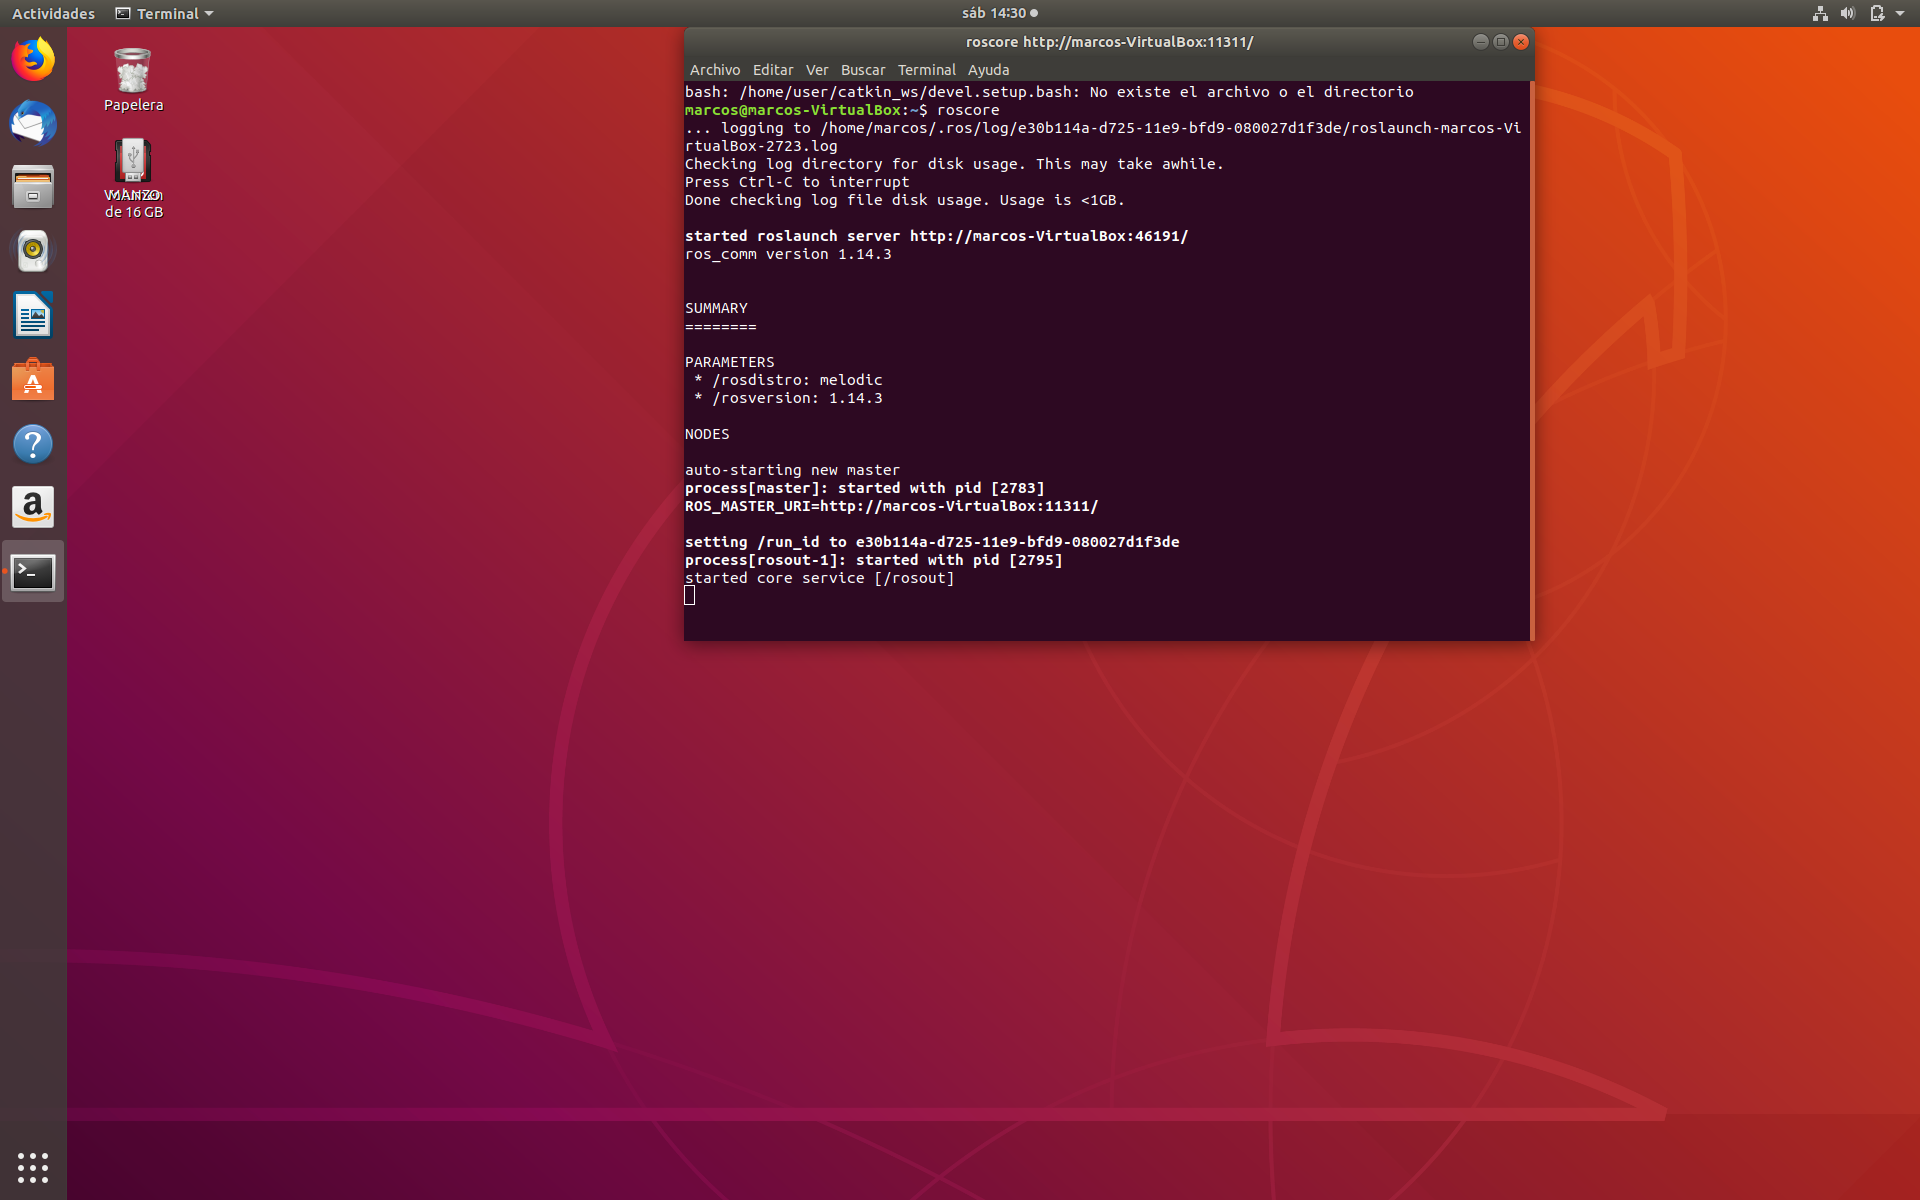
\includegraphics[scale=.15]{link21.png}
\end{center}
\begin{center}
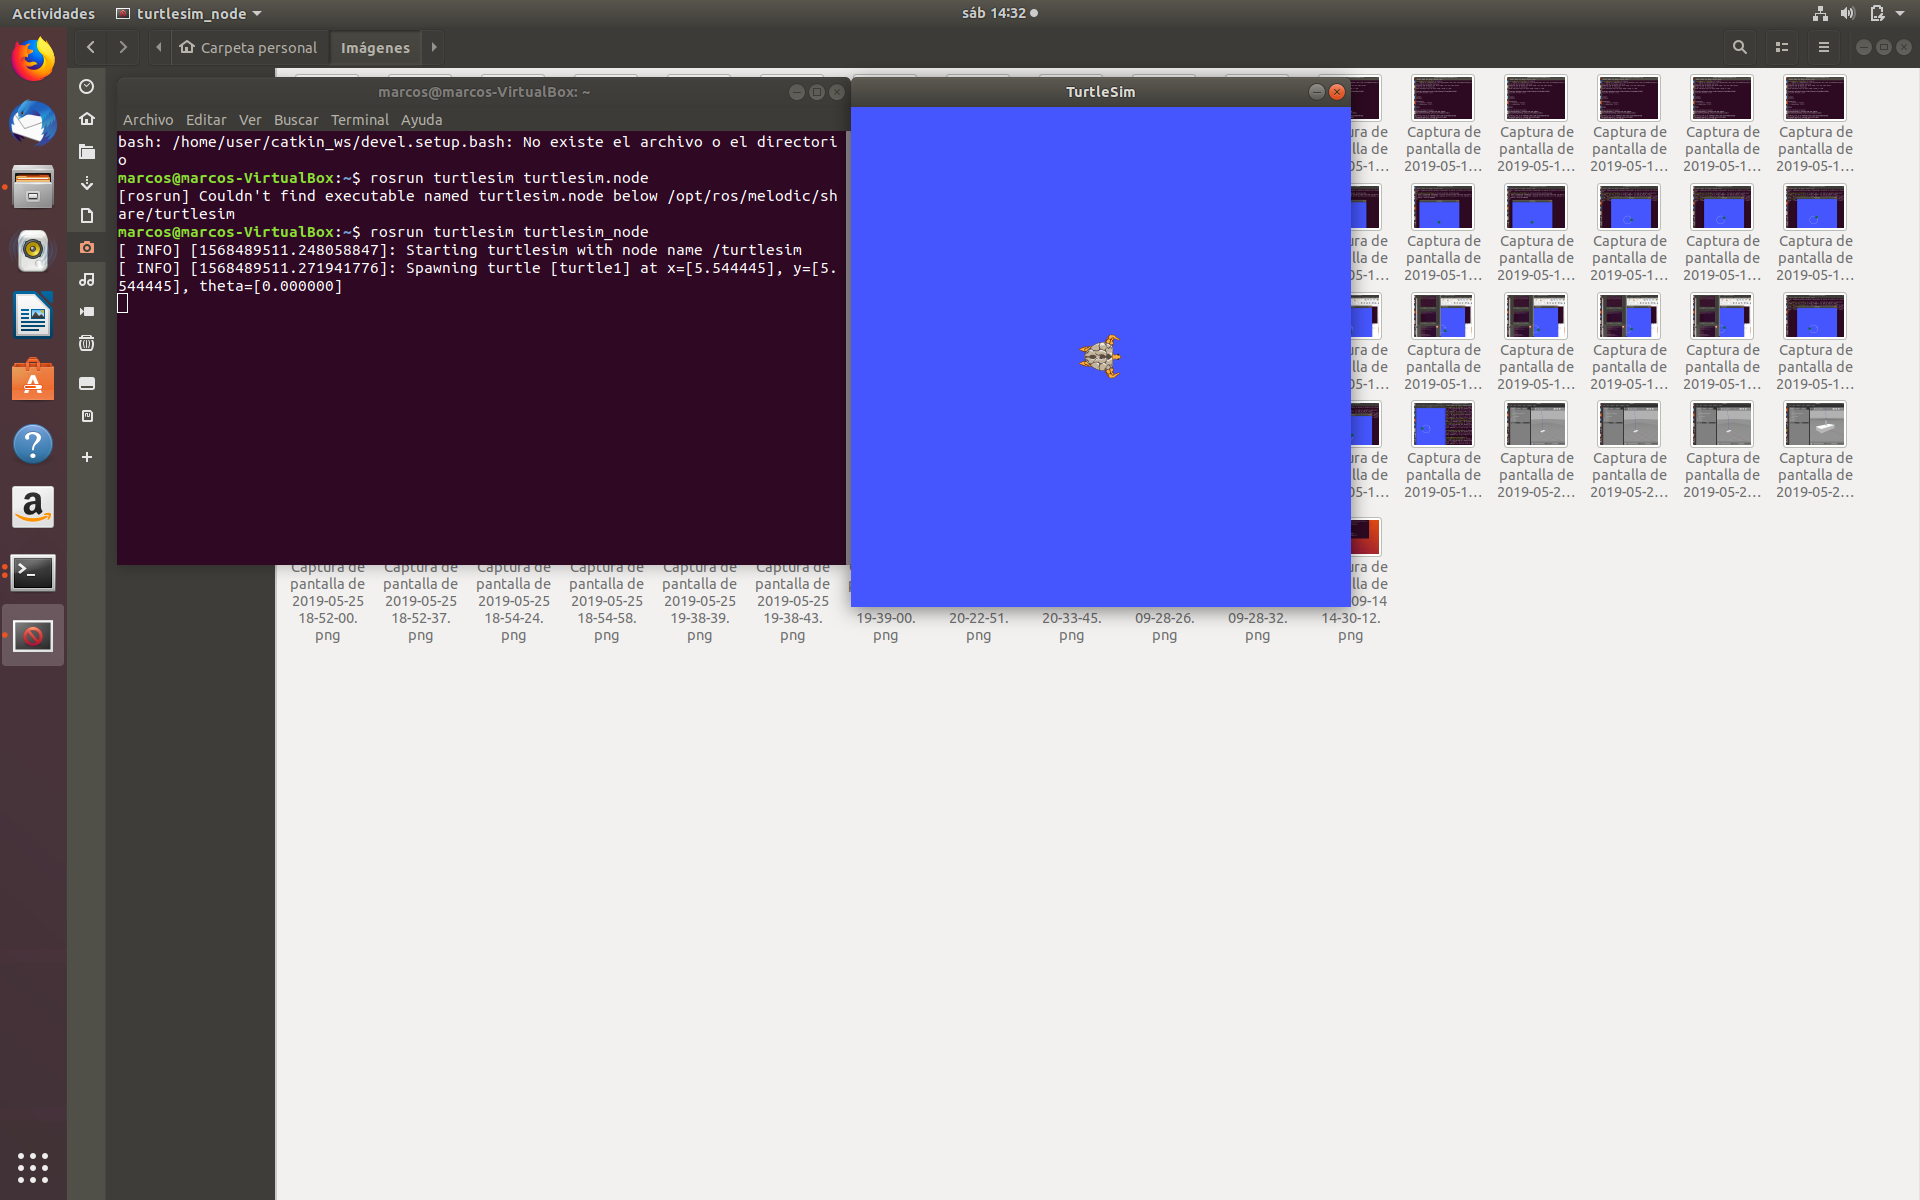
\includegraphics[scale=.15]{link23.png}
\end{center}
\section{Conclusión}
ROS se perfila como una opción mundial para el avance de la programación robótica. En este sentido, resulta importante desarrollar competencias en el manejo de tal sistema. Pero de lo que inconscientemente ROS me enseño, fue su complicada forma de instalación, ya que tienes que estas investigando y leyendo diferentes blogs para saber que es compatible y que ya no. Tiene un grado de dificultad saber que versiones son las necesarias. Al igual que Latex, ya es necesario a esta altura investigar por nuestra cuenta y navegar por internet para investigar cuales son nuestras dudas desde como instalar hasta como escribir un documneto en Latex.


\section{Referencia}
[1]Kick-Starting Robot Programming Using ROS,Joseph, Lentin,Robot Operating System (ROS) for Absolute Beginners,pages127--170,2019, publisher{Springer}.

\bibliographystyle{unsrt}
\bibliography{Torres.bib}



\begin{center}
Gracias.
\end{center}


\end{document}